\chapter{Cálculo de matriz de covarianzas: síntesis hardware y optimización con HLS}

\section{Introducción}
Se ha expuesto a grandes rasgos en el capítulo anterior cómo es el proceso de obtención de vectores normales a una superficie definida por una nube de puntos. Además, se ha indicado qué parte de dicho proceso será objeto de optimización con hardware digital, la obtención de matrices de covarianzas.

En el presente capítulo se exponen las diferencias entre el código original y el modificado para que sea sintetizable en hardware. Tras esto, se indicarán las optimizaciones realizadas sobre el código modificado y la generación de la IP (Intellectual Property) para el posterior trabajo con ella.




\section{Algoritmo original de estimación de matrices de covarianzas}

En la librería PCL se puede encontrar el método que permite calcular la matriz de covarianzas asociada a un punto estudiado y sus vecinos dentro de la nube de puntos original sobre la que se desean obtener los vectores normales\cite{calculo_covarianzas}. Sobre éste se realizarán las modificaciones pertinentes para que el código resultante sea sintetizable en hardware.

Como se ha explicado previamente, el método \textit{computeMeanAndCovarianceMatrix} recibe como argumentos la nube de puntos original como \textit{cloud}, un vector que contiene los índices de los puntos que forman una vecindad entorno al punto estudiado en la iteración actual como \textit{indices} y \textit{covariance\_matrix} y \textit{centroid} para guardar respectivamente la matriz de covarianzas y el centroide obtenidos.

\begin{lstlisting}[language=C++,breaklines]
  template <typename PointT, typename Scalar> inline unsigned int
pcl::computeMeanAndCovarianceMatrix (const pcl::PointCloud<PointT> &cloud,
                                     const std::vector<int> &indices,
                                     Eigen::Matrix<Scalar, 3, 3> &covariance_matrix,
                                     Eigen::Matrix<Scalar, 4, 1> &centroid)
{
\end{lstlisting}

Aparece la librería Eigen para crear una matriz llamada \textit{accu} en la que guardar resultados intermedios. Se comprueba si el atributo \textit{is\_dense} de la nube \textit{cloud} es \textit{true} o \textit{false} para llevar a cabo las mencionadas operaciones intermedias de diferentes maneras. En cualquiera de los casos, se recorre todo el vector de índices para obtener los resultados adecuados en \textit{accu} que posteriormente se divide entre el número de elementos del vector \textit{indices}.


\begin{lstlisting}[language=C++,breaklines]

  Eigen::Matrix<Scalar, 1, 9, Eigen::RowMajor> accu = Eigen::Matrix<Scalar, 1, 9, Eigen::RowMajor>::Zero ();
  size_t point_count;
  if (cloud.is_dense)
  {
    point_count = indices.size ();
    for (size_t i = 0; i <= point_count; ++i)
    {
      accu [0] += cloud[indices[i]].x * cloud[indices[i]].x;
      accu [1] += cloud[indices[i]].x * cloud[indices[i]].y;
      accu [2] += cloud[indices[i]].x * cloud[indices[i]].z;
      accu [3] += cloud[indices[i]].y * cloud[indices[i]].y;
      accu [4] += cloud[indices[i]].y * cloud[indices[i]].z;
      accu [5] += cloud[indices[i]].z * cloud[indices[i]].z;
      accu [6] += cloud[indices[i]].x;
      accu [7] += cloud[indices[i]].y;
      accu [8] += cloud[indices[i]].z;
    }
  }
  else
  {
    point_count = 0;
    for (size_t i = 0; i <= indices.end(); ++i)
    {
      if (!isFinite (cloud[indices[i]]))
        continue;

      ++point_count;
      accu [0] += cloud[indices[i]].x * cloud[indices[i]].x;
      accu [1] += cloud[indices[i]].x * cloud[indices[i]].y;
      accu [2] += cloud[indices[i]].x * cloud[indices[i]].z;
      accu [3] += cloud[indices[i]].y * cloud[indices[i]].y;
      accu [4] += cloud[indices[i]].y * cloud[indices[i]].z;
      accu [5] += cloud[indices[i]].z * cloud[indices[i]].z;
      accu [6] += cloud[indices[i]].x;
      accu [7] += cloud[indices[i]].y;
      accu [8] += cloud[indices[i]].z;
    }
  }

  accu /= static_cast<Scalar> (point_count);
 \end{lstlisting}
 
Por último, se almacenan en \textit{centroid} y \textit{covariance\_matrix} los resultados finales del algoritmo.
 
 \begin{lstlisting}[language=C++,breaklines]
  centroid[0] = accu[6]; centroid[1] = accu[7]; centroid[2] = accu[8];
  centroid[3] = 1;
  covariance_matrix.coeffRef (0) = accu [0] - accu [6] * accu [6];
  covariance_matrix.coeffRef (1) = accu [1] - accu [6] * accu [7];
  covariance_matrix.coeffRef (2) = accu [2] - accu [6] * accu [8];
  covariance_matrix.coeffRef (4) = accu [3] - accu [7] * accu [7];
  covariance_matrix.coeffRef (5) = accu [4] - accu [7] * accu [8];
  covariance_matrix.coeffRef (8) = accu [5] - accu [8] * accu [8];
  covariance_matrix.coeffRef (3) = covariance_matrix.coeff (1);
  covariance_matrix.coeffRef (6) = covariance_matrix.coeff (2);
  covariance_matrix.coeffRef (7) = covariance_matrix.coeff (5);

  return (static_cast<unsigned int> (point_count));
}
\end{lstlisting}



\section{Algoritmo modificado e integración en Vivado HLS}
Se ha decidido seleccionar el cálculo de la matriz de covarianzas explicado en la figura \ref{fig:compute_computeMean} para su optimización puesto que se reduce a operaciones con vectores y matrices que no requieren el uso de librerías específicas a diferencia del cálculo de las componentes del vector normal que necesita utilizar Eigen y complica la optimización.

No solamente se mostrará a continuación el código modificado sino que se indicará su integración en el programa Vivado HLS, del cual se hace uso para la síntesis en hardware y su optimización.

En primer lugar se crea un nuevo proyecto en Vivado HLS y se selecciona la FPGA con la que se trabaja en el presente trabajo, la PYNQ-Z1 modelo xc7z020clg400-1.

A la hora de integrar en HLS el algoritmo de cálculo de matrices de covarianzas, se hace uso de tres ficheros de texto:

\begin{list}{•}
\item[•] \textit{normal.cpp}: Es el código de PCL modificado que permite extraer matrices de covarianzas, además de ciertos aspectos añadidos pertenecientes a la optimización y síntesis hardware.
\item[•] \textit{normal\_tb.cpp}: Se trata de un test bench que comprueba el correcto funcionamiento de normal.cpp pues compara resultados reales con simulados. Cabe destacar aquí que se ha modificado ligeramente la librería PCL para que tras cada cómputo de una matriz de covarianzas y centroide, éstos se guarden en un fichero de texto cada uno para así tener acceso a estos resultados en cualquier momento.
\item[•] \textit{normal.hpp}: Es el conjunto de herramientas y librerías necesarias para normal.cpp y normal\_tb.cpp
\end{list}

\subsubsection{normal.cpp}

Las modificaciones realizadas sobre el método \textit{computeMeanAndCovarianceMatrix} son las siguientes:

\begin{list}{•}
\item[•] Puesto que en la síntesis de hardware digital no se pueden tener variables de tamaño no fijo, es decir, no se pueden manejar herramientas de asignación dinámica de memoria, los argumentos \textit{cloud} y \textit{indices} tienen un tamaño máximo del cual se utiliza el necesario según las variables \textit{num\_points} y \textit{num\_indices} que se refieren a las dimensiones de la nube y vector de índices respectivamente.

\item[•] todas las líneas que comienzan por ``\#pragma'' indican la creación de buses en los que agrupar variables para su interpretación en hardware. En concreto, el bus A contiene las entradas del algoritmo y el bus B las salidas. 

\item[•] Se ha eliminado la comprobación del atributo \textit{is\_dense} de la nube de puntos de entrada puesto que se no trabaja con nubes que contienen puntos cuya posición no esté determinada por un valor finito.

\item[•] Todas las instancias pertenecientes a la clase Eigen han sido suprimidas y sustituidas por variables del tipo correspondiente como es en el caso de la variable \textit{covariance\_matrix} que es una matriz de tipo flotante.

\end{list}

 \begin{lstlisting}[language=C++,breaklines]
 #include "normal.h"

int compute (volatile float covariance_matrix[3][3],
		volatile float centroid[4],
		volatile float cloud[MAXPOINTS][3],
		volatile int indices[MAXINDICES],
		int num_points,
		int num_indices){

	//entradas
	#pragma HLS INTERFACE s_axilite port=cloud bundle=BUS_A
	#pragma HLS INTERFACE s_axilite port=indices bundle=BUS_A
	#pragma HLS INTERFACE s_axilite port=num_indices bundle=BUS_A
	#pragma HLS INTERFACE s_axilite port=num_points bundle=BUS_A

	//salidas
	#pragma HLS INTERFACE s_axilite port=covariance_matrix bundle=BUS_B
	#pragma HLS INTERFACE s_axilite port=centroid bundle=BUS_B
	#pragma HLS INTERFACE s_axilite port=num_points bundle=BUS_B
	#pragma HLS INTERFACE s_axilite port=return bundle=BUS_B

	float accu[9]={0};


	compute_label0:for(int i = 0;i<num_indices;i++){
		accu[0] += cloud[indices[i]][0] * cloud[indices[i]][0];
		accu[1] += cloud[indices[i]][0] * cloud[indices[i]][1];
		accu[2] += cloud[indices[i]][0] * cloud[indices[i]][2];
		accu[3] += cloud[indices[i]][1] * cloud[indices[i]][1];
		accu[4] += cloud[indices[i]][1] * cloud[indices[i]][2];
		accu[5] += cloud[indices[i]][2] * cloud[indices[i]][2];
		accu[6] += cloud[indices[i]][0];
		accu[7] += cloud[indices[i]][1];
		accu[8] += cloud[indices[i]][2];
	}

	for(int i = 0;i<9;i++){
		accu[i]/=num_indices;
	}
	centroid[0] = accu[6];
	centroid[1] = accu[7];
	centroid[2] = accu[8];
	centroid[3] = 1;

	covariance_matrix[0][0] = accu [0] - accu [6] * accu [6];
	covariance_matrix[0][1] = accu [1] - accu [6] * accu [7];
	covariance_matrix[0][2] = accu [2] - accu [6] * accu [8];
	covariance_matrix[1][1] = accu [3] - accu [7] * accu [7];
	covariance_matrix[1][2] = accu [4] - accu [7] * accu [8];
	covariance_matrix[2][2] = accu [5] - accu [8] * accu [8];

	covariance_matrix[1][0] = accu [1] - accu [6] * accu [7];
	covariance_matrix[2][0] = accu [2] - accu [6] * accu [8];
	covariance_matrix[2][1] = accu [4] - accu [7] * accu [8];


	return num_points;
}
\end{lstlisting}

\subsubsection{normal\_tb.cpp}

Las operaciones realizadas por el test bench se resumen en los siguientes puntos:

\begin{list}{•}
\item Creación de variables tales como dos matrices de tipo float que almacenan la nube (\textit{cloud}) y la matriz de covarianzas (\textit{covariance\_matrix}), vector de tipo float que almacena los índices de los puntos de la nube que forman una vecindad (\textit{indices}), vector de tipo float que almacena las coordenadas del centroide del conjunto de puntos que forman una vecindad (\textit{centroid}) y las ya mencionadas \textit{num\_points} y \textit{num\_indices}.

\item La nube de puntos está almacenada en un fichero de formato .txt por lo que se efectúa su lectura y se almacena en \textit{cloud}. Se hace lo mismo con un fichero de texto que contiene los índices de los puntos que forman una vecindad: se leen de un fichero de texto y se almacenan en \textit{indices}.

\item Se llama al método implementado en \textit{normal.cpp} para obtener los resultados deseados en las variables \textit{covariance\_matrix} y \textit{centroid}

\item se leen los ficheros de texto que contienen la matriz de covarianzas y el centroide calculados por el código original gracias a la modificación de la librería PCL previamente mencionada y se compara con los resultados obtenidos por el código modificado.
\end{list}

Se muestra en la imagen \ref{fig:resultados_hls} que el valor de la matriz de covarianzas y el centroide calculados con el código original y modificado efectivamente coinciden. Esto se consigue con la herramienta de simulación del código, es decir, se corre el test bench que utiliza el algoritmo desarrollado en \textit{normal.cpp}

\begin{figure}
\centering
\includegraphics[scale=0.7]{resultados_hls}
\caption{comparación de matriz de covarianzas y centroide obtenidos con Vivado HLS y PCL. ``covariance matrix before'' y ``centroid before'' indican que se muestran la matriz de covarianzas y el centroide inicializados a cero.}\label{fig:resultados_hls}
\end{figure}



\subsubsection{normal.hpp}

Se incluyen las librerías necesarias y se declaran las variables y el método que se usan en normal\_tb.cpp y normal.cpp además de definir las constantes ``MAXPOINTS'' y ``MAXINDICES'' que son las dimensiones máximas de la nube de puntos y el vector de índices como ya se ha discutido previamente sobre la imposibilidad de utilizar memoria dinámica en hardware.

\begin{lstlisting}[language=C++,breaklines]
#include <stdio.h>
#include <iostream>
#include <math.h>
#include <fstream>
#include <stdlib.h>
#include <vector>

#include <hls_stream.h>
#include <ap_axi_sdata.h>

#define MAXPOINTS 970
#define MAXINDICES 15



int compute(volatile float covariance_matrix[MAXPOINTS][3],
		volatile float centroid[4],
		volatile float cloud[MAXPOINTS][3],
		volatile int indices[MAXINDICES],
		int num_points,
		int num_indices);
\end{lstlisting}


\subsection{Generación de síntesis e IP}

Sabiendo que los resultados obtenidos con PCL y HLS coinciden, se procede a la ejecución de la síntesis para estimar el uso de los recursos de los que dispone la FPGA. Así pues, en la figura \ref{fig:resultados_sintesis_hls} se puede ver un uso del 10\% de la memoria disponible así como un 11\% y 29\% de flip flops y lookup tables respectivamente. El recurso más variable es la memoria en forma de block RAM o BRAM ya que depende del tamaño de la nube con la que se trabaja y por tanto la cantidad de información que tiene que manejar la FPGA. En la figura \ref{fig:resultados_sintesis_hls2} se aprecian resultados referentes a tiempos y latencia en forma de ciclos de reloj necesarios para ejecutar el algoritmo.

\begin{figure}[!htb]
\minipage{0.48\textwidth}
  \includegraphics[width=\linewidth]{resultados_sintesis_hls}
  \caption{Estimación de utilización de recursos de la FPGA.}\label{fig:resultados_sintesis_hls}
\endminipage\hfill
\minipage{0.48\textwidth}
  \includegraphics[width=\linewidth]{resultados_sintesis_hls2}
  \caption{Estimación de latencia y tiempos en la FPGA.}\label{fig:resultados_sintesis_hls2}
\endminipage\hfill
\end{figure}

Tras comprobar que la FPGA tiene un uso correcto de sus recursos se puede exportar el Register Transfer Level (RTL) y generar la IP mediante la opción ``export RTL'' especificando que sea descrita en VHDL. Este bloque IP, que se llamará ``compute'', se utilizará en Vivado para configurar la FPGA para la aplicación del presente trabajo, optimización del cálculo de matriz de covarianzas.

\begin{figure}
\centering
\includegraphics[scale=0.7]{export_RTL}
\caption{Exportación de RTL y generación de IP.}\label{fig:export_RTL}
\end{figure}

\section{Integración de la IP en Vivado}
Teniendo exportada la IP que permite calcular matrices de covarianzas mediante hardware, se ha de configurar la FPGA con dicha funcionalidad.

Se crea un nuevo proyecto en el programa Vivado y se genera un diagrama de bloques como se muestra en la figura \ref{fig:diagrama_vivado} sobre el cual se destaca:
\begin{itemize}
\item[•] \textbf{processing\_system7\_0}: Se trata del Processing System (PS) explciado en el capítulo 2.
\item[•] \textbf{compute\_0}: Es la IP generada con Vivado HLS y que ha sido importada a Vivado.
\item[•] \textbf{system\_ila\_0}: Se trata del Integrated Logic Analyzer (ILA) y se encarga de tareas de debug haciendo uso de los propios recursos de la FPGA, puesto que los buses A y B contienen las entradas y salidas de \textbf{compute\_0} y las cuales se quieren controlar y observar.
\end{itemize}


\begin{figure}
\centering
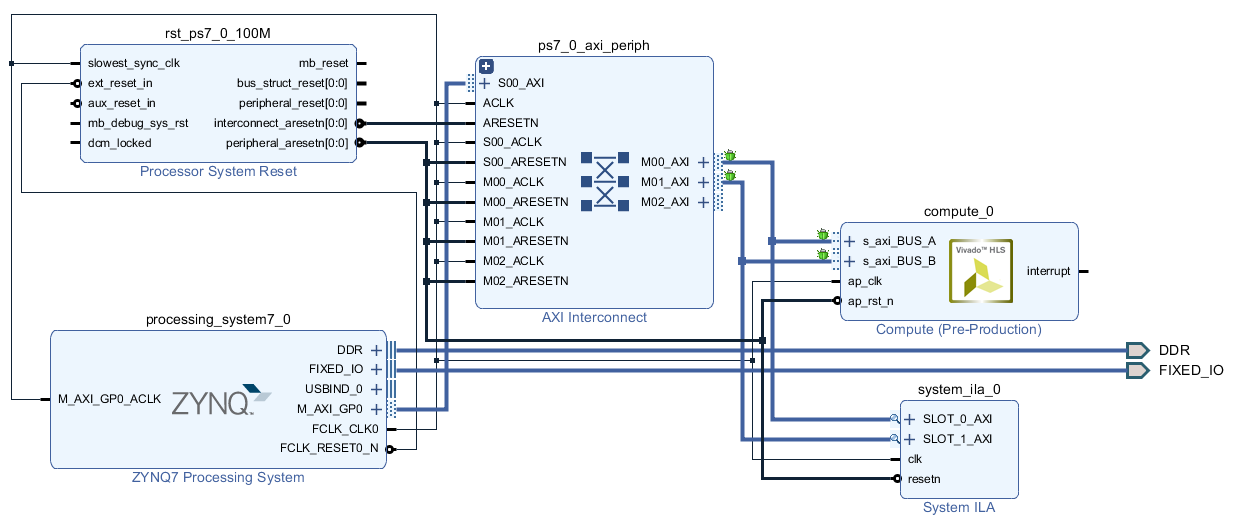
\includegraphics[scale=0.55]{diagrama_vivado}
\caption{Diagrama de bloques de la FPGA Pynq-Z1 y la IP de cálculo de matrices de covarianzas.}\label{fig:diagrama_vivado}
\end{figure}

Una vez comprobado que el diagrama es correcto se puede proceder a la generación del archivo de configuración que se cargará en la FPGA, el ``bitstream''. Esto se hace de forma automática y ofrece como resultado, a parte del mencionado archivo, una visión, en azul claro, de los recursos utilizados de la capa de aplicación de la FPGA tal y como se aprecia en la figura \ref{fig:recursos_fpga}

\begin{figure}
\centering
\includegraphics[scale=0.7]{recursos_fpga}
\caption{Recursos hardware utilizados para implementar la IP generada en Vivado HLS.}\label{fig:recursos_fpga}
\end{figure}

\section{Comprobación del funcionamiento de la IP sobre la FPGA}
El último paso antes de poder hacer uso de la IP ya configurada en la FPGA es comprobar que funciona adecuadamente sobre ésta. Para ello, utilizando Vivado, se exporta el hardware generado y los drivers para controlar la IP a un kit de desarrollo software (Software Deevlopement Kit o SDK) basado en Eclipse mediante el cual se puede hacer uso de la IP generada en Vivado HLS gracias a los mencionados drivers. 

En el SDK se abre un nuevo proyecto vacío basado en el hardware exportado desde Vivado, es decir, la configuración de la FPGA y que se encuentra en el entorno de trabajo del kit de desarrollo. Para utilizar la IP cobre la FPGA se crea un archivo en lenguaje C que sirve de test bench para comprobar el correcto funcionamiento del cálculo de matrices de covarianzas. Este archivo es muy similar al test bench ya creado y explicado en Vivado HLS pero tiene ciertas diferencias:

\begin{itemize}
\item[•] Hay que comprobar que el cálculo de matrices de covarianzas da al mismo resultado ejecutándose mediante software (código en C compilado) y hardware (utilizando los drivers y los recursos hardware de la FPGA, es decir, su lógica programable PL) A efectos de cómo escribir el test bench solamente afecta al desdoblamiento de variables, esto es, se necesitan dos variables que almacenen la matriz de covarianzas (y otros resultados finales y/o intermedios) en una de ellas la calculada mediante software y la otra mediante hardware.
\end{itemize} 


\section{Conclusiones}


